\chapter{Computational Spectral Unmixing}\label{chap:Csu}

\section{Introduction}

In \Cref{chap:Afssic}, I argued that spectral classification is the goal of spectral imaging in most cases. However, in certain situations the analyst is interested in quantifying the presence of several materials in a single spatial location from a \gls{mixed spectrum}. Mixed spectra can occur when the sensor is part of a high-altitude platform such as an unmanned aerial vehicle (UAV) or satellite. The large standoff distances between the ground and the instrument result in large spatial resolutions. For example, in the Hyperion Imaging Spectrometer, which is satellite based, the spatial resolution is 30 meters \cite{folkman2001eo}. One cannot reasonably expect a single material to always occupy that large of an area. \Gls{spectral unmixing} is any procedure which attempts to take the measured spectrum of a mixed pixel and decompose it into a set of constituent spectra called the \glspl{endmember} and a set of corresponding fractions called the \glspl{fractional abundance}. 

Traditional spectral unmixing requires several seperate steps to quantify the fractional abunances. The isomorphic sensor must spatially or spectral scan object scene, building the spectral datacube piece by piece. At each step, the restricted aperture or wavelength range rejects a significant fraction of the availiable light. A post-processing step is then used to reduce the size of the data to reduce the computational load. Finally an inversion step is used to compute the fractional abundances. Intuitively, the advantages of computational sensing discussed throughout this dissertation should be able to ameliorate some of the design trade-offs in traditional spectral unmixing.

In this chapter, I will talk about my efforts to apply the techniques of computational sensing to directly estimate the \gls{fractional abundance} without the need to reconstruct the spectral datacube. I will introduce a computational spectral imaging architecture called the \gls{lcsi}. I will then provide simulation results that demonstate the advantage of spectral unmixing over traditional spectral imaging architectures, by leveraging the Fellgett and Jacquinot advantage with sparsity promoting optimization algorithms. Results from a proof-of-principle experiment demonstrate the promise of computational spectral unmixing. 

\section{The Linear Mixing Model}

There are two main reasons why mixed spectra occur \cite{keshava2002spectral, keshava2003survey}. First, if the spatial resolution of the sensor is low enough, separate materials can jointly occupy the \acrfull{fov} of a single pixel, the resulting spectral measurement is a combination of the constituent spectra, see \Cref{fig:linearAndNonlinearMixing}(a). In this case, one can imagine the object scene as a \emph{checkerboard} mixture: light from the illumination source scatters or reflects from only one of the materials before being observed by the sensor, multiple scattering between materials are ignored. The second reason for mixed pixels occurs when different materials are combined into a homogeneous mixture, see \Cref{fig:linearAndNonlinearMixing}(b). In this case, mixed spectra are not caused by poor spatial resolution, they are inherent to the nature of the scene. For the purposes of this chapter I will focus on the first case, mixed spectra arise due to the spatial resolution. 

\begin{figure}
	\centering
	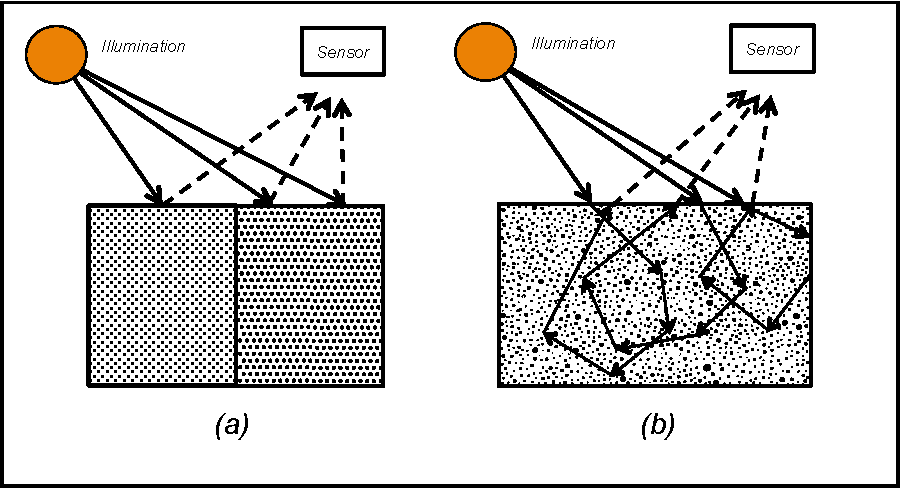
\includegraphics[scale=0.85]{linearAndNonlinearMixing.pdf}
	\captionof{figure}[Linear versus Non-Linear Mixing]{(a) Illustration of linear mixing where incident solar radiation reflects from a surface and the surface consists of distinct materials. (b) Illustration of nonlinear mixing where incident solar radiation encounters an intimate mixture of materials, reflecting or scattering multiple times before being reflected toward the spectral image sensor.}
	\label{fig:linearAndNonlinearMixing}
\end{figure}

When mixed spectra occur due to the spatial resolution limitation of the instrument, the fractional abundance is linearly proportional to the relative area of each material. This is called the linear mixing model \gls{lmm}, where the mixed spectrum can be written as 
%
\begin{equation}
\mb{f} = \sum_{r=1}^{N_{R}} x_r \mb{s}_r + \mb{e} = \mb{S} \mb{x}  + \mb{e}
\end{equation}
%
where $\mb{f}$ is the \gls{mixed spectrum}, $\mb{s}_r$ is the $r^{th}$ endmember spectrum, $\mb{S}$ is a matrix in which the columns are the endmember spectra, $\mb{x}$ is the fractional abundance vector, and $N_{R}$ is the number of endmembers in the endmember library, each spectra has \gls{numspecchan} spectral channels. In the \gls{lmm}, the interactions between distinct endmembers are assumed to be neglible \cite{clark1984reflectance}. 

There are two contraints imposed by the physics of the situation. Intuitively we should expect that the fractional abundance should be equal to or larger than zero. This is the \emph{nonnegativity} constraint:
%
\begin{equation}
	x_r \geq 0.
\end{equation}
%
We should also expect that if energy is conserved, i.e. there is no absorption of light, then the \gls{fractional abundance} should sum to one. This is the \emph{additivty} constraint:
%
\begin{equation}
	\sum_{r = 1}^{N_{R}} x_r = 1
\end{equation}


\subsection{Unmixing in Traditional Spectral Imaging}

In traditional spectral imaging, the spectral datacube is first isomorphically acquired by the instrument before any unmixing step is performed. Often a \gls{dimensionality reduction} step is used to reduce the computational burden of processing the spectral datacube \cite{keshava2002spectral, keshava2003survey}. If the endmembers are unknown, an \gls{endmember determination} step is executed. Finally, the \gls{inversion} step is used to estimate the fractional abundances. 

Notable data reduction algorithms include \acrfull{pca} and \acrfull{mnf}. As described in Chapter 2, \gls{pca} is applied to the measured data and finds the basis which decorrelates the data. In \gls{pca} one typically observes a steadily decreasing signal-to-noise ratio as the principal compenent number increases \cite{green1988transformation}. However, this is not always the case, it equates variance with information and is based on the assumption that the data structure can be described by a multi-dimensional normal distribution \cite{philpot2015mnf}. In \gls{mnf}, the algorithm attempts to order the components in terms of \gls{snr} which consists of two seperate \gls{pca} rotations and a noise whitening step. \gls{mnf} requires estimation of the noise covariance matrix in addition to the covariance of the data.

%A non-statistical technique for dimensionality reduction is the optical real-time adaptive spectral identification system (ORASIS) \cite{bowles2007optical}, which is a series of steps that identify a subset of representative, or exemplar, pixels that convey the variables in a scene. When a new pixel is collects from the scene, a spectrum is compared to each examplar pixel using this angle metrix. If it is sufficently different then it is added to the set. Then using a modified Gram-Schmidt process, an orthogoal basis is created and a new dimension is added until the every exemplar can be represented well within a certain tolerances \cite{keshava2003survey}. 

The inversion step actually estimates the \gls{fractional abundance}. There are a variety of inversion techniques which actually attempt to estimate the fractional abundance vector. Many are based on minimizing the squared error and attempt to enforce additivity or non-negativity \cite{keshava2003survey, lawson1995solving}. An example of a statistical non-parameteric technique attempts to minimize the variance of the estimator \cite{steven1993fundamentals}. There are also various algorithms based on \acrfull{map}, \acrfull{mle}, and clustering which can be used for spectral unmxing. Unfortunately, we cannot explore each inversion technique, due to there prevalence, I will use least-squares based inversion techniques when comparing computational spectral unmixing techniques. 





\section{Architecture}

In this research, two seperate architectures are used for spectral unmixing. The first architecture is the \gls{afssi-c} which was described in depth in \Cref{chap:Afssic}. The second architecture is an \acrfull{lcos} based spectral imager, called the \gls{lcsi}, which allows for an extremely compact instrument called the \gls{lcsi}, see \Cref{fig:lcsiArchi}. The system provides a programmable spectral filter, which can be independently addressed at each physical pixels of the \gls{slm}. The device consists of an array of micro cells of liquid crystal on a reflecting layer \cite{lazarev2012lcos}. Each layer of liquid crystal can be modeled as a thin retarder plate. Since most birefringent phase retarders are sensitive to wavelength, this element combined with a polarizing beam splitter or a linear polarizer produces a wavelength dependent transmission pattern, a spectral filter, which modulates the input spectra \cite{yuan2015compressive}.

\begin{figure}
	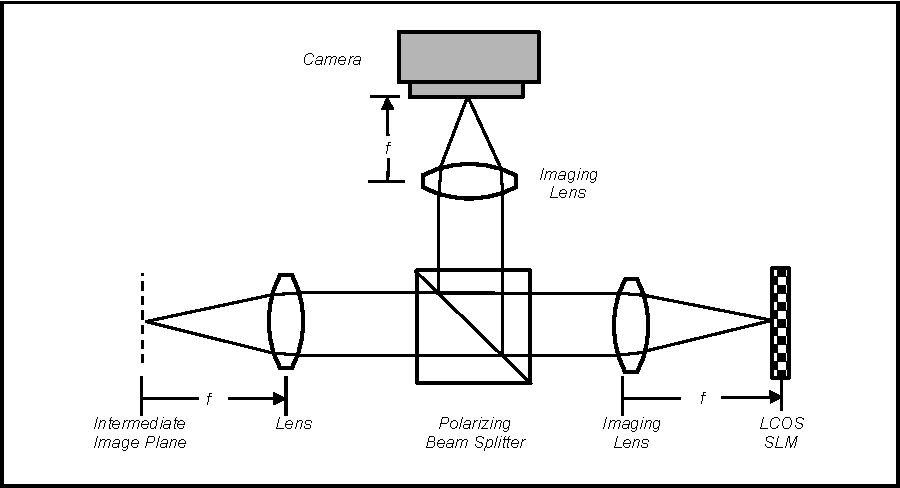
\includegraphics[scale=1.0]{lcsiArchi.pdf}
	\captionof{figure}[LCOS Based Spectral Imager]{The LCOS Spectral Imager. Light from the intermediate image plane is collimated. A polarizing beam splitter passes p-polarized light and rejects s-polarized light. Upon reflection of the LCOS SLM, the polarization state is changed to some elliptical polarization state. Only the s-polarized portion of the elliptical polarization is reflected toward the upper part where it is imaged onto a scientific camera. The intensity of the light that is passed depends on birefringence created by the programmable LCOS.}
	\label{fig:lcsiArchi}
\end{figure}

%\subsection{How the LCOS Creates Spectral Filters}
% Imagine an incident monochromatic plane wave traveling in the z-direction with a Jones polarization vector 
% \begin{equation}
% \mbh{a} = 
% 	\begin{bmatrix}
%     	a_{x}  \\
%     	a_{y} e^{ i \phi  }  \\
%    \end{bmatrix}
% \end{equation}
% %
% where $\phi$ is the phase differene between the x and y axes \cite{milster2013notes}. The full plane wave for the electric field can be written as

% \begin{equation}
% \mb{E} = A \exp \left[ \mb{k} \cdot \mb{r} - \omega t \right] \mbh{a}
% \end{equation}
% %
% where there leading $A$ is a complex constant that adjusted for amplitude and absolute phase shift.
% %
% \begin{equation}
% 	\mb{k} = k \mbh{k} = k \ap{ \alpha \mbh{x} + \beta \mbh{y} + \gamma \mbh{z} }
% \end{equation}
% %
% is the propagation vector with wavenumber $k = 2\pi /\ \lambda$ and direction cosines $\ap{\alpha, \beta, \gamma}$.

% Transmitting through the polarizing beam splitter only passes horizontally polarized light

% \begin{equation}
% 	\begin{bmatrix}
% 		a_x \\
% 		0 
% 	\end{bmatrix}
% 	=
% 	\begin{bmatrix}
% 		1 & 0 \\
% 		0 & 0
% 	\end{bmatrix}
% 	\begin{bmatrix}
% 		a_x  \\
% 		a_y e^{ i \phi  }
% 	\end{bmatrix}
% 	\label{eq:jonesAfterPBS1}
% \end{equation}

% The \gls{lcos} in our architecture is a phase only reflective type. Liquid crystal is used because it has the ability change birefringence $\Delta n$ when an electric field is applied. Birefringence is defined as 
% %
% \begin{equation}
% 	\Delta n = n_e - n_0
% \end{equation}
% %
% where $n_0$ is the ordinary refractive index and $n_e$ is the extraordinary refractive index \cite{zhang2014fundamentals}. By changing the electric field in the cell the $\Delta n$ is changed. 

% Birefringence is utilized to create retardation plates. These retardation plates serve to change the polarization state of input light. If one aligns the retardation plate so that the x polarized light is incident on the ordinary refractive index and the y polarized light is incident onto the ordinary refractive index then x and y polarizations are phase shifted by
% %
% \begin{equation}
% 	\eta = \frac{2 \pi}{\lambda} \left[ n_e\ap{\lambda} - n_o \ap{\lambda} \right] T
% \end{equation}
% %
% where $T$ is the physical thickness of the plate, where the $ n_e \ap{ \lambda } $ and $ n_o \ap{\lambda} $ are index of refraction of the extraordinary and ordinary waves which are wavelength dependant functions \cite{milster2013notes}. 

%The general Jones matrix for an arbitrary birefringent material as a retardation plate is
%
%\begin{equation}
%	\begin{bmatrix}
%		M_{11} & M_{12} \\
%		M_{21} & M_{22}
% 	\end{bmatrix}
% 	=
% 	\begin{bmatrix}
% 		e^{i \eta/2} \cos^2 \theta + e^{-i \eta/2} \sin^2 \theta & \ap{ e^{i \eta/2} - e^{-i \eta/2} } e^{-i \phi} \cos \theta \sin \theta \\
% 		\ap{ e^{i \eta/2} - e^{-i \eta/2} } e^{i \phi} \cos \theta \sin \theta & e^{i \eta/2} \sin^2 \theta + e^{-i \eta/2} \cos^2 \theta
% 	\end{bmatrix}
% 	\label{eq:arbJonesMatrix}
% \end{equation}
% %
% where the relative phase retardation between the fast and slow axes is given by $\eta = \phi_y - \phi_x$, $\theta$ is the orientation of the fast axis with respect to the x-axis, and $\phi$ is the circularity. Thus after propagating from the LCOS the Jones Vector is written as
% %
% \begin{equation}
% 	\begin{bmatrix}
% 		a_x M_{11} \\
% 		a_x M_{21}
% 	\end{bmatrix}	
% \end{equation}
% %
% finally the vertical polarization (y) is reflected by the polarizing beam splitter towards the camera
% %
% \begin{equation}
% 	\begin{bmatrix}
% 		0 \\
% 		a_x M_{21}
% 	\end{bmatrix}	
% \end{equation}

% Where the intensity is pro



% The phase shift can be used to change the polarization state of the light. For example, when linearly polarized light at 45 degrees goes through a phase shift of $\Delta = \lambda / 2$ the polarized light will rotate to vertical. However, this is a special case and in general the output light will be elliptically polarized. When elliptically polarized light is incident onto a linear polarizer, only linearly polarized light is passed, the intensity of the light passed however depends on the relative amplitude and phase of the x and y polarizations of the incident light \cite{milster2013notes}. 

Unfortunately, a full discussion of polarization is out of the context of this disseration. The important point is that for light of a single wavelength, the \gls{lcos} can manipulate the polarization, which in general is not linearly polarized. Placing a polarizer after light has been reflected from the \gls{lcos} will force the transmitted light to be linearly polarized but at an intensity depedent on the projection of the input polarization. The ordinary and extraordinary index of refraction depdend on the wavelength of light. Thus phase shift imparted to the two polarizations will be wavelength depdent. Passing non-monochromatic light to an \gls{lcos} and then a linear polarizer will impart a wavelength depdent intensity. In short, the \gls{slm} provides polarization and wavelength depdent transmission patterns to encoded the spectral datacube \cite{tsai2015spatial}.


\subsection{Forward Model}

The forward model for the \gls{lcsi} is similar to the forward model for the \gls{afssi-c} presented in \Cref{ssec:afssicForwardModel}, except now one does not need to account include dispersion when imaging from the input plane to the LCOS and from the LCOS to the \gls{fpa} of the camera. I will thus skip the derivation of the forward model and simply present the final equation for the measurement value at pixel $n$ and $l$ from the camera:
%
\begin{align} 
	\Gamma_{nl} &= \sum_{n^\prime l^\prime} \iiint \mbox{rect} \left( \frac{x}{\Delta} - l, \frac{y}{\Delta} - n \right) \mbox{rect} \left( \frac{x}{\Delta} - l^\prime , \frac{y}{\Delta} - n^\prime \right) \notag \\
 	&\qquad \times T_{n^\prime l^\prime} \ap{\lambda} D_0 \left( x, y; \lambda \right) dx \, dy \, d\lambda.
\end{align}
%
Notice that there is no dispersion constraint like the one created in the \gls{afssi-c} or a joint spatial-spectral contraints like in the \gls{cassi}. The \gls{lcos} creates dispersion by the very nature of wavelength dependant birefringence. If one so choose to, one can simply treat each pixel in the image as completely indepdent from neighboring pixels. This greatly simplifies the analysis. 

Similar to the \gls{afssi-c} we can further simplify this by imagining a discrete spectral density, the spectral datacube. The discretized source spectral datacube is $D$, and then the detector signal $\Gamma$ is a result of spectral filter created by the PBS-LCOS combination where spectral filter $T$ acting on the pixelated source is
%
%
\begin{equation}
	\Gamma_{n,l} = \sum^{N_{\lambda}-1}_{c = 0} T_{n,l,c} D_{n,l,c} \,
\end{equation}
%
%
which shows the measurement at each pixel being the inner product of the source spectrum and the spectral filter created by the PBS-LCOS combination. In a single spatial location, this reduces to a simple inner product
%
\begin{equation}
	g_m = \mb{h}_m^{T} \mb{f} 
\end{equation}
%
where the subscript $m$ represents the $m^{\text{th}}$ measurement step and $\mb{f}$ the true spectrum at that pixel. For a sequence of measurements this simplies to 
%
\begin{equation}
	\mb{g} = \mb{H} \mb{f}
\end{equation}
%
where the $m^{th}$ row of $\mb{H}$ is $\mb{h}_m^T$ and $\mb{g}$ is an $m \times$1 vector, $\mb{f}$ is the ground truth mixed spectrum
%
\begin{equation}
	\mb{f} = \mb{S}\mb{x}
\end{equation}
%
Thus for a sequence of noisy measurements at a single pixel
%
\begin{equation}
	\mb{g} = \mb{H}\mb{S}\mb{x} + \mb{e} = \mb{A}\mb{x} + \mb{e}
\end{equation}\label{eq:csuForwardModel}
%
where $\mb{H}$ is an $N_m \times N_{\lambda}$ matrix, $\mb{S}$ is the endmember library which is an $N_{\lambda} \times N_{R}$ matrix, $\mb{x}$ is the fractional abundance vector which an $N_R \times 1$ vector, $\mb{e}$ is the additive noise which is a $N_m \times 1$ vector. If I define
%
\begin{equation}
	\mb{A} = \mb{H} \mb{S}.
\end{equation}
%
One can think of $\mb{H}$ as the sensing matrix and $\mb{S}$ as the representation matrix as discussed in \Cref{sec:compressiveSesing}.


\section{Solving the Inverse Problem}

For this work I chose to use the least-squares estimator (LSE)
%
\begin{equation}
	\mbh{x} = \ap{ \mb{A}^T \mb{A} }^{-1} \mb{A}^T \mb{g}
\end{equation}\label{eq:lseEquationChap5}
%
to demonstrate the advantage provided by multiplexing without using compressive sensing based algorithms. To demonstrate compressive sensing approaches, I will used the built-in MATLAB \texttt{lasso} function which attempts to minimize the $\ell_1$ regularized least-squares objective function 
%
\begin{equation}
	\mbh{x} = \argminA_{\mb{x}} \: \| \mb{Ax} - \mb{g} \|_{2}^{2} + \tau \| \mb{x} \|_1
	\label{eq:l1reglsV2}
\end{equation}
%
in order to find fractional abundances that are sparse. 

In the traditional spectral imager, the fractional abundance is estimated after the spectral datacube is acquired. In our work, the fractional abundance can be estimated after each measurement step. However, since we need a way to compare our results to traditional spectral imaging, we can use the tunable filter architectures for a baseline comparision. The tunable filter acquires a single wavelength over the entire field-of-view and thus allows us to obtain measurements in a time sequential manner. This means that we can use the LSE to get an idea of how a traditional spectral imaging architecture would perform.

As I mentioned earlier, remote sensing the fractional abundance vector $\mbh{x}$ tends to be sparse: the number of endmembers in the library is much larger than number of endmembers that are actually present in the mixed spectrum $N_{R} > \| \mb{x} \|_0$. Therefore, one can invoke the techniques designed for compressive sensing to find solutions that are sparse.

\section{Prior work}

NOT REALLY SURE WHERE TO PUT THIS SECTION!!

\subsection{Prior Efforts in Computational Spectral Unmixing}

Several researchers have shown promising results in applying compressive sensing to spectral unmixing using a modified single-pixel camera architecture \cite{li2012compressive}. They demonstrated the ability to reconstruct the fractional abundance planes without the need to explicitly reconstruct the spectral datacube. In this approach, the object scene is imaged onto a \gls{dmd} and then a condensor lens focuses the reflected light into a whiskbroom spectrometer. One can think of this architecture as a set of parallel single-pixel cameras each operating at a different spectral channel, with the constraint that each \gls{dmd} must display the same pattern. This architecture does not code the spectral dimension of the spectral datacube. The researchers demonstrated compressive unmixing by minimizing the total variation (TV) of the endmember images while enforcing the nonnegativity constraint. 

In another effort, researchers use the \acrfull{cassi} architecture to perform compressive sensing on the spectral datacube and solve the $\ell_1$-regularized least squares problem (lasso in regression) to promote sparsity in the fractional abundances \cite{monsalve2015spectral}. Due to the nature of the single-disperser \gls{cassi} architecture, the researchers are forced to solve a larger joint-inference problem to preform spectral unmixing. 

\subsection{Prior efforts using LCOS Computational Spectral Imaging}

Several groups have previously demonstrated computational spectroscopy and spectral imaging results using variations of liquid crystal technology. The first instance, in 2012, used a single-pixel liquid crystal device to demonstrate compressive spectroscopy and exhibited a 10$\times$ reduction in the number of measurements compared to a traditional ismorphic spectrometer \cite{august2013compressive}. Shortly after in 2013, a demonstration of a compressive spectral imager using an \gls{lcos} \gls{slm} was published which jointly coded spatial and spectral features \cite{zhu2013coded}. In 2015, an \gls{lcos} based hyperspectral imaging sensor demonstrated blind compressive sensing, using a Bayesian approach to dictionary learning \emph{in situ} \cite{yuan2015compressive}. That same year, a miniture ultraspectral imaging system based on a custom built liquid crystal cell, which applies the same spectral filter to each spatial location, demonstrated the ability to reconstruct gigapixel spectral datacubes with an order of magnitude reduction in measurement steps compared to isomorphic systems \cite{august2016miniature}. However, to our knowledge, no one has ever attempted to perform direct spectral unmixing using an \gls{lcos} based device. 


\section{Designing Spectral Filters for Unmixing}

I will now discuss spectral filter design and selection for computational spectral unmixing. 

In \Cref{chap:Afssic}, I have shown that adaptive code design significantly improved classification results. While in \Cref{chap:Scout}, I have shown that using careful optimizing of codes can improve reconstruction results in a compressive sensor. For the \gls{afssi-c} architecture, I will discuss both adaptive and non-adaptive approaches to spectral coding and for the \gls{lcsi} architecture I will discuss a heurstic approach to selecting spectral filters. 

For this work, I will quantify the unmixing error using the \acrfull{rmse} between the estimated fractional abundance $\mbh{a}$ and the ground truth fractional abundance $\mb{a}$

\begin{equation}
	RMSE =  \left[ \frac{1}{N_R} \sum_{r = 1}^{N_{R}} \ap{ \hat{a}_r - a_r }^2 \right]^{\frac{1}{2}}
\end{equation}

The \gls{afssi-c} has the ability to display psuedo-arbitrary spectral filters with the restriction of using binary codes $ \{ -1, +1 \}$ using the \gls{dmd}. If one is interested in using the \gls{afssi-c} architecture for computational spectral \textbf{imaging}, then the dispersion constraint discussed in \Cref{sec:adaptiveClassficiationAlgo} must be considered in any code design scheme. 

In the \gls{afssi-c}, one can emulate a tunable filter spectrometer by measuring one spectral channel at time, i.e. turn on one mirror per measurement step. In this case, the measurement matrix is equal to the identity matrix $\mb{H} = \mb{I}$. Combining the tunable filter approach with the LSE produces what one should expect from a traditional isomorphic spectral imager to conduct spectral unmixing.

We can also use random binary codes to achieve a multiplexed measurement. As demonstrated in the \gls{afssi-c}, one should expect that sampling multiple spectral channels per measurement should reduce the unmixing error. The spectrum can then be estimated by combining the multiplexed measurements with a traditional, non-sparsity promoting, estimator such as the LSE to demonstrate the performance gained by simply collecting more light per measurement step. However, pairing an compressive sensing algorithm with a random binary code can produce even better unmixing results by enforcing the sparsity. 

\subsection{Adaptive Unmixing Algorithm For the AFSSI-C}\label{sec:unmixingAlgo}

We developed an adaptive unmixing algorithm for creating spectral filters is which inspired by the one used for creating spectral filters in spectral classification: a modified version of \gls{pca} is used to create adaptive spectral filters. This algorithm begins with the spectral library which consist of the each endmember spectra $\mb{S}$. Initially, before any measurements are made, the estimated fractional abundances of each endmember are assumed to be the same: 
%
\begin{equation}
	\mbh{a}_{m=0} = 
	\begin{bmatrix}
	\frac{1}{N_R} \\
	\frac{1}{N_R} \\
	\vdots \\
	\frac{1}{N_R}
	\end{bmatrix}
\end{equation}
%
where $N_R$ is the number of endmembers. The subscript denotes the $m^{th}$ measurement step, so before any measurement is made, $m=0$. Then each endmember in the spectral library is then weighted by the square of their respective estimated fractional abundance
%
\begin{equation}
	\mb{S}_w = 
	\begin{bmatrix}
		\hat{a}_1^2 \mb{s}_1 & \hat{a}_2^2 \mb{s}_2 & \hdots & \hat{a}_{N_R}^2 \mb{s}_{N_R}
	\end{bmatrix}
	\label{eq:weightedSpectralLibrary}
\end{equation}
%
Then the eigenvectors of the unnormalized covariance matrix of the weighted spectral library are computed
%
\begin{equation}
	X_m = \mb{S}_w \mb{S}_w^T 
\end{equation}
%
These are the principal component vectors. Where the first principal component corresponds to the direction of largest variance and so on. Initially, for the first measurement, the algorithm chooses the first principal component for the spectral filter $\mb{h}_{m=1} = \mb{p}_1$. The measurement is then recorded
%
\begin{equation}
	g_{m=1} = \mb{h}_{m=1}^{T} \mb{f} + e_{m}
\end{equation}
%
A simulated ``guess'' measurement based on the current estimated fractional abundance is also computed. 
\begin{equation}
	\gamma_{m=1} = \mb{h}_{m=1}^{T} \mb{S} \mbh{a}_{m=0}
\end{equation}
%
notice that the guess measurement does not include any simulated noise. Remember $\mb{S}$ denotes the original spectral library matrix, not the weighted spectral library matrix. After the measurement is recorded, the $\ell_2$ norm of the difference between the guess measurement and the actual measurement is recorded:
%
\begin{equation}
	\xi_m = \| \gamma_m - g_m \|_2 
\end{equation}
%
The fractional abundance is then estimated. While the MATLAB \texttt{lasso} function is used to estimate the fractional abundance, in practice, the LSE is used for the first measurement step since the function requires atleast two rows or entries to run. 

The spectral library is then reweighted using \Cref{eq:weightedSpectralLibrary}. Again the principal components are recomputed. For the second measurement step, $m=2$ the second principal component is used for the spectral filter. After the measurement has been recorded, the  $\ell_2$ norm of the difference between the guess measurement and the actual measurement is computed again $\xi_m$. 

%Again the weighted spectral library is recomputed as well as the principal components. 

This continues until either two things happen: 
\begin{enumerate}
	\item If the current $\ell_2$ norm of the difference between the guess and the actual measurement exceeded the last $\ell_2$ norm of the difference between guess and actual measurement
	%
	\begin{equation}
		\xi_m > \xi_{m-1} - \frac{\sigma}{2}
	\end{equation}	
	%
	where $\sigma$ is the standard deviation of the system noise, which is assumed to be \gls{awgn}.

	\item Used the sixth principal component.
\end{enumerate}

when either of these two conditions are met, the loop resets to using the first principal component again. I constrained the algorithm to only use the first six principal components, because I noticed that the unmixing preformance is optimized when limited to only the first six principal components. Intuitively, this may be occuring because higher principal components tend exhibit lower SNR or because the spectra in the library do not exhibit significant high frequency features. 

In summary, if the difference between the guess measurement and the actual measurement is improving, the algorithm continues to select the next principal component from the weighted spectral library library until it reaches the six principal component. Otherwise, if the difference has not changed by a certain amount then or the sixth principal component has been used, the algorithm goes back to the first principal component. This algorithm is called the switching \gls{swpca}. It is important to note that as of yet, this algorithm does not consider the dispersion constraint of the \gls{afssi-c}, and therefore is more appropriate for the single pixel version, the \gls{afss}. The MATLAB code which simulates \gls{swpca} is found in Appendix \ref{app:adaptiveUnmixAlgo}.


\subsection{Hybrid Spectral Filters for the LCSI}

The spectral filters produced by the \gls{lcsi} architecture are constrained by the physics of the birefringence dispersion created by the \gls{lcos}. For our particular model, the Holoeye PLUTO LCOS SLM, the spectral filter is changed by sending a different grayscale value to the green channel of the video output (Holoeye allows their SLM to be connected like a second monitor). Since there are 255 grayscale values, there are 255 different spectral filters, see \Cref{fig:slmSpectralFiltersVisible}. 

Since one is not able to design the spectral filters individually, the next best thing is to choose which spectral filters should be used at each measurement step. Intuitively, one can imagine that using the same spectral filter or similar spectral filters over and over will lead to a measurement matrix $\mb{H}$ where the rows are not incoherent enough to satisfy the \acrfull{rip}. 

For my experiment, I will compare several methods of choosing the spectral filters. The first method is simply selecting them at random from a discrete uniform distribution between 1 and 255, while constraining the selections to prevent using the same spectral filter more than once. However, additional prior knowledge about the statistics of the endmembers are not exploted in random filter selection. 

The second technique attempts to use \gls{pca} to select the spectral filters. The algorithm computes the principal components of the endmembers (spectral library) and then select the spectral filters which most closely resemble the principal component vector $\mb{p}$ using an angle metric:
%
\begin{equation}
	\mb{h} = \argmaxA_{\mb{h}} \: \left\{ \frac{ \mb{p} }{ \| \mb{p} \| } \cdot \frac{ \mb{h} }{ \| \mb{h} \|  } \right\}.
\end{equation}
%
For the $m^{th}$ measurement, the spectral filter whose dot product is largest with the $m^th$ principal component of the endmember matrix is selected. However, using all the principal components actually increases the unmixing error after a certain amount of measurement steps. This occurs because after a certain number of principal components the spectral filters are similar or the spectral filter being selected is simply the same one over and over again. Thus, we created a hybrid spectral filter selection technique that uses \gls{pca} to select the first several spectral filters and then uses psuedo-random selections after a certain number of measurement steps. This balances the ability of \gls{pca} to chose spectral filters that improve the unmixing error at the initial measurement steps while using random selections to ensure the measurement matrix is incoherent enough to satisfy the \gls{rip}.

The hybrid approach to selecting the spectral filters is further extended to use a more advanced version of \gls{pca} called \acrfull{mnf} transform. \gls{mnf} was originally developed to remove noise from multispectral satellite images \cite{green1988transformation} and attempts to select a basis which orders the signal-to-noise ratio of the MNF components. However, \gls{mnf} is also used for Blind Signal Seperation (BSS), which is the seperation of a set of source signals from a set of mixed signals \cite{hundley2001solution}. Instead of computing the principal components, I compute the maximum noise fraction components of the spectral library. I specifically used the noise adjusted principle component analysis (NAPCA) algorithm to compute the MNF of the spectra library which is found in \cite{hundley2001solution}. The algorithm associates rapidly varying parts of the spectral library with

\begin{figure}
	\centering
	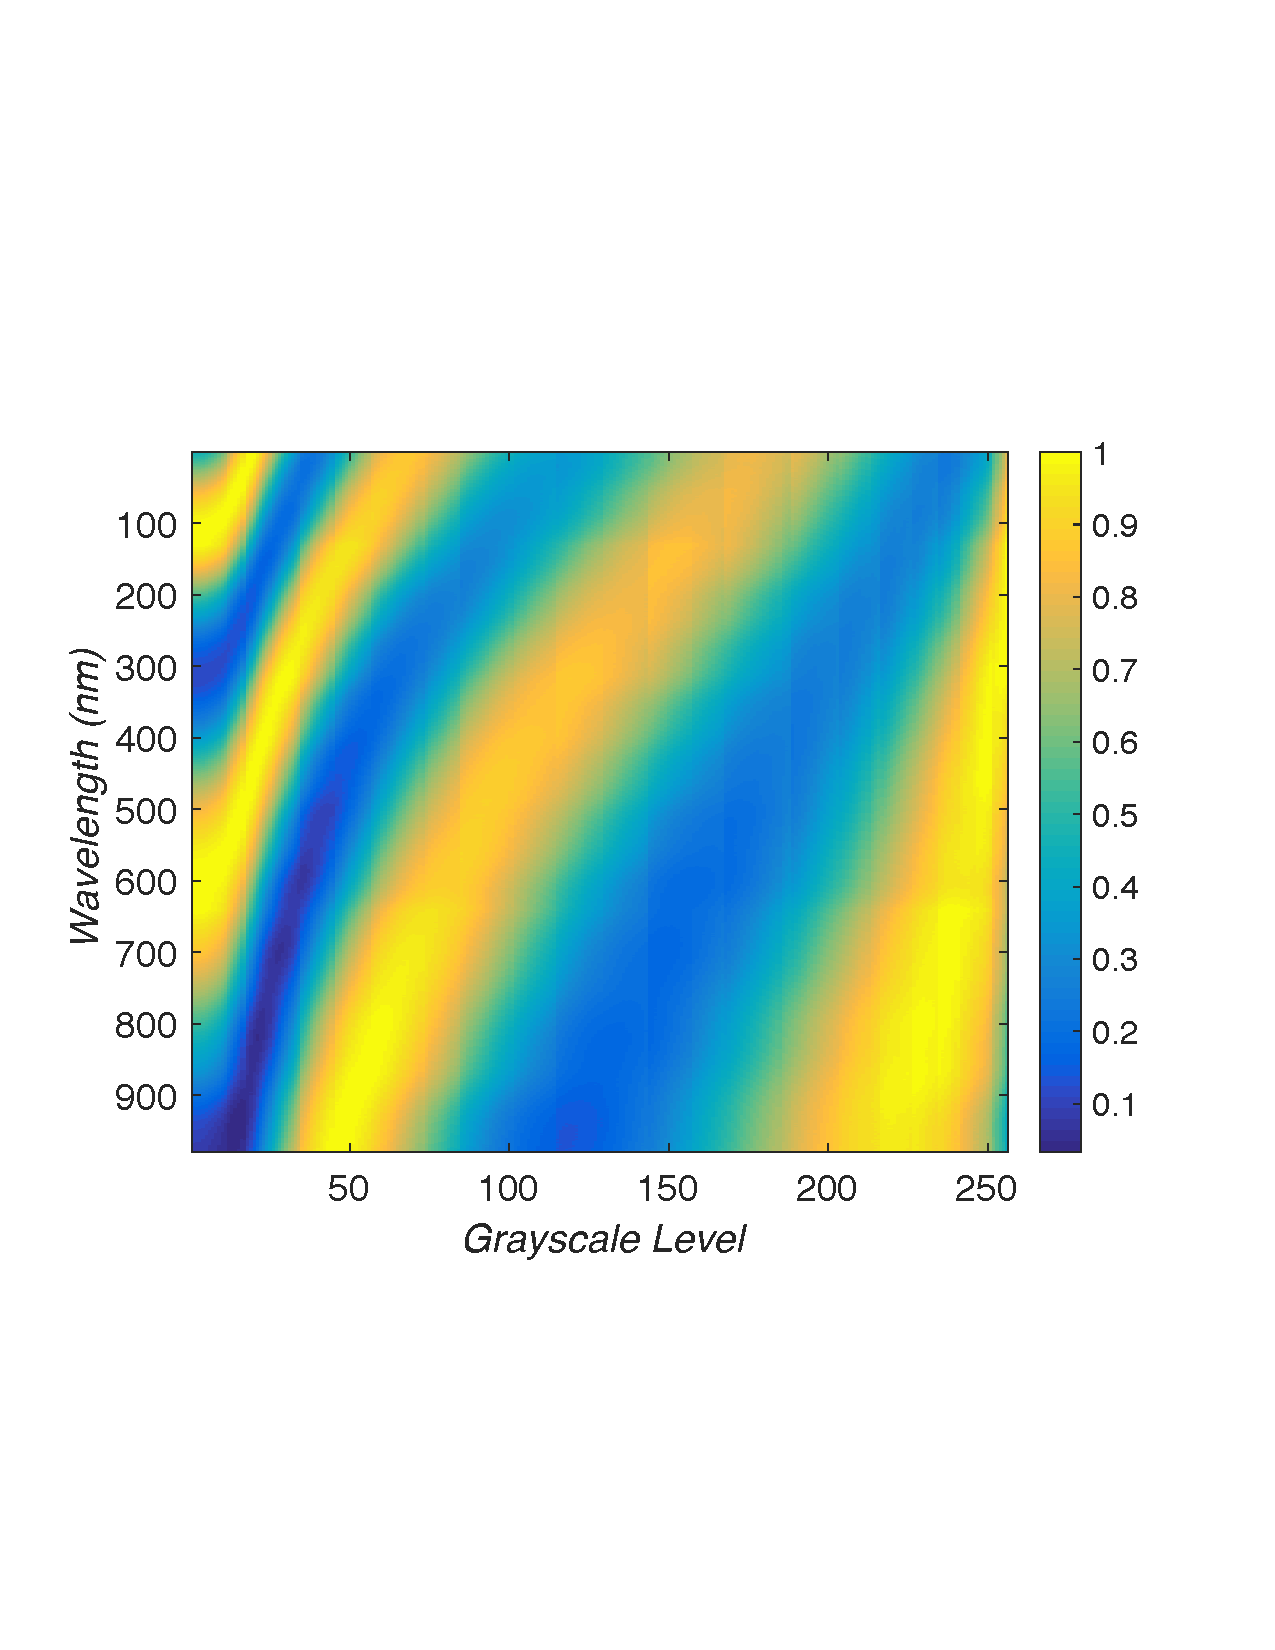
\includegraphics[scale=0.75]{slmSpectralFiltersVisible.pdf}
	\captionof{figure}[The Spectral Filters created by the Holoeye PLUTO SLM and polarizing beam splitter]{The spectral filters created by the Holoeye PLUTO SLM and polarizing beam splitter. Each column is the a spectral filter at a particular grayscale level which is sent to the PLUTO SLM. }
	\label{fig:slmSpectralFiltersVisible}
\end{figure}


\subsection{Simulation Results}

In order to quantify the improvements that multiplexing and sparse solutions provide over traditional spectral unmixing, I performed monte carlo simulations over five different noise levels SNR = $10^-2$ to $10^2$. As a basis of comparison, I first simulated the tunable filter architecture with the least squares estimation (LSE).


\begin{figure}
	\centering
	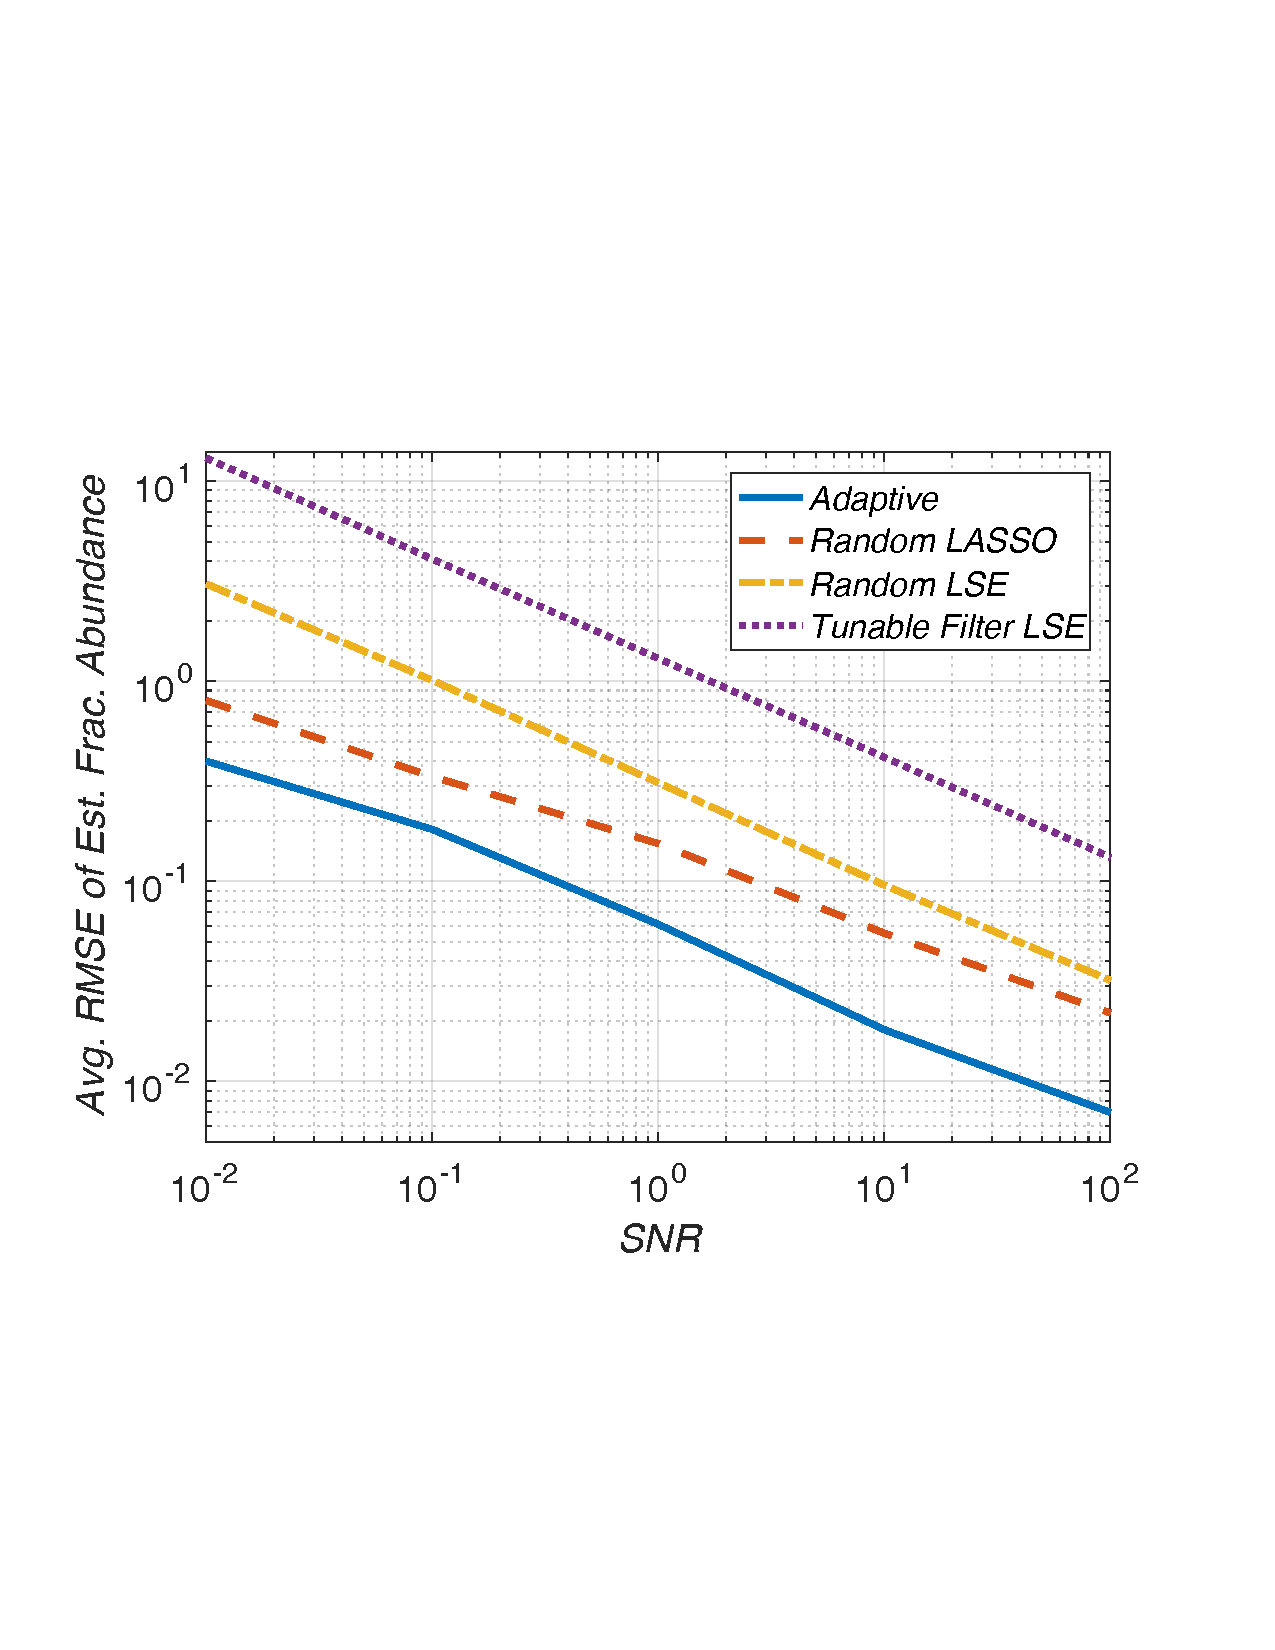
\includegraphics[scale=0.75]{unmixingTechniquesComparison.pdf}
	\captionof{figure}[Comparison of Spectral Unmixing Techniques for the AFSSI-C at five different SNR levels]{A comparison of spectral unmixing techniques for the AFSSI-C at five different SNR levels. The y-axis represents the average RMSE of the estimate fractional abundance. The x-axis represents the signal-to-noise in the measurements. The tunable filter LSE refers to the average unmixing performance if one were to use a tunable filter spectral imaging architectures with least squares estimation to estimate the fractional abundance. The random LSE line refers to the improvement in spectral unmixing This shows the improvement that multiplexing provides over simple tunable filter spectral imaging using the least squares estimator (LSE). Then using the multiplex advantage and algorithms that promote sparsity when the fractional abundance is known to be sparse, one can significantly outperform }
	\label{fig:unmixingTechniquesComparison}
\end{figure}


\begin{figure}
	\centering
	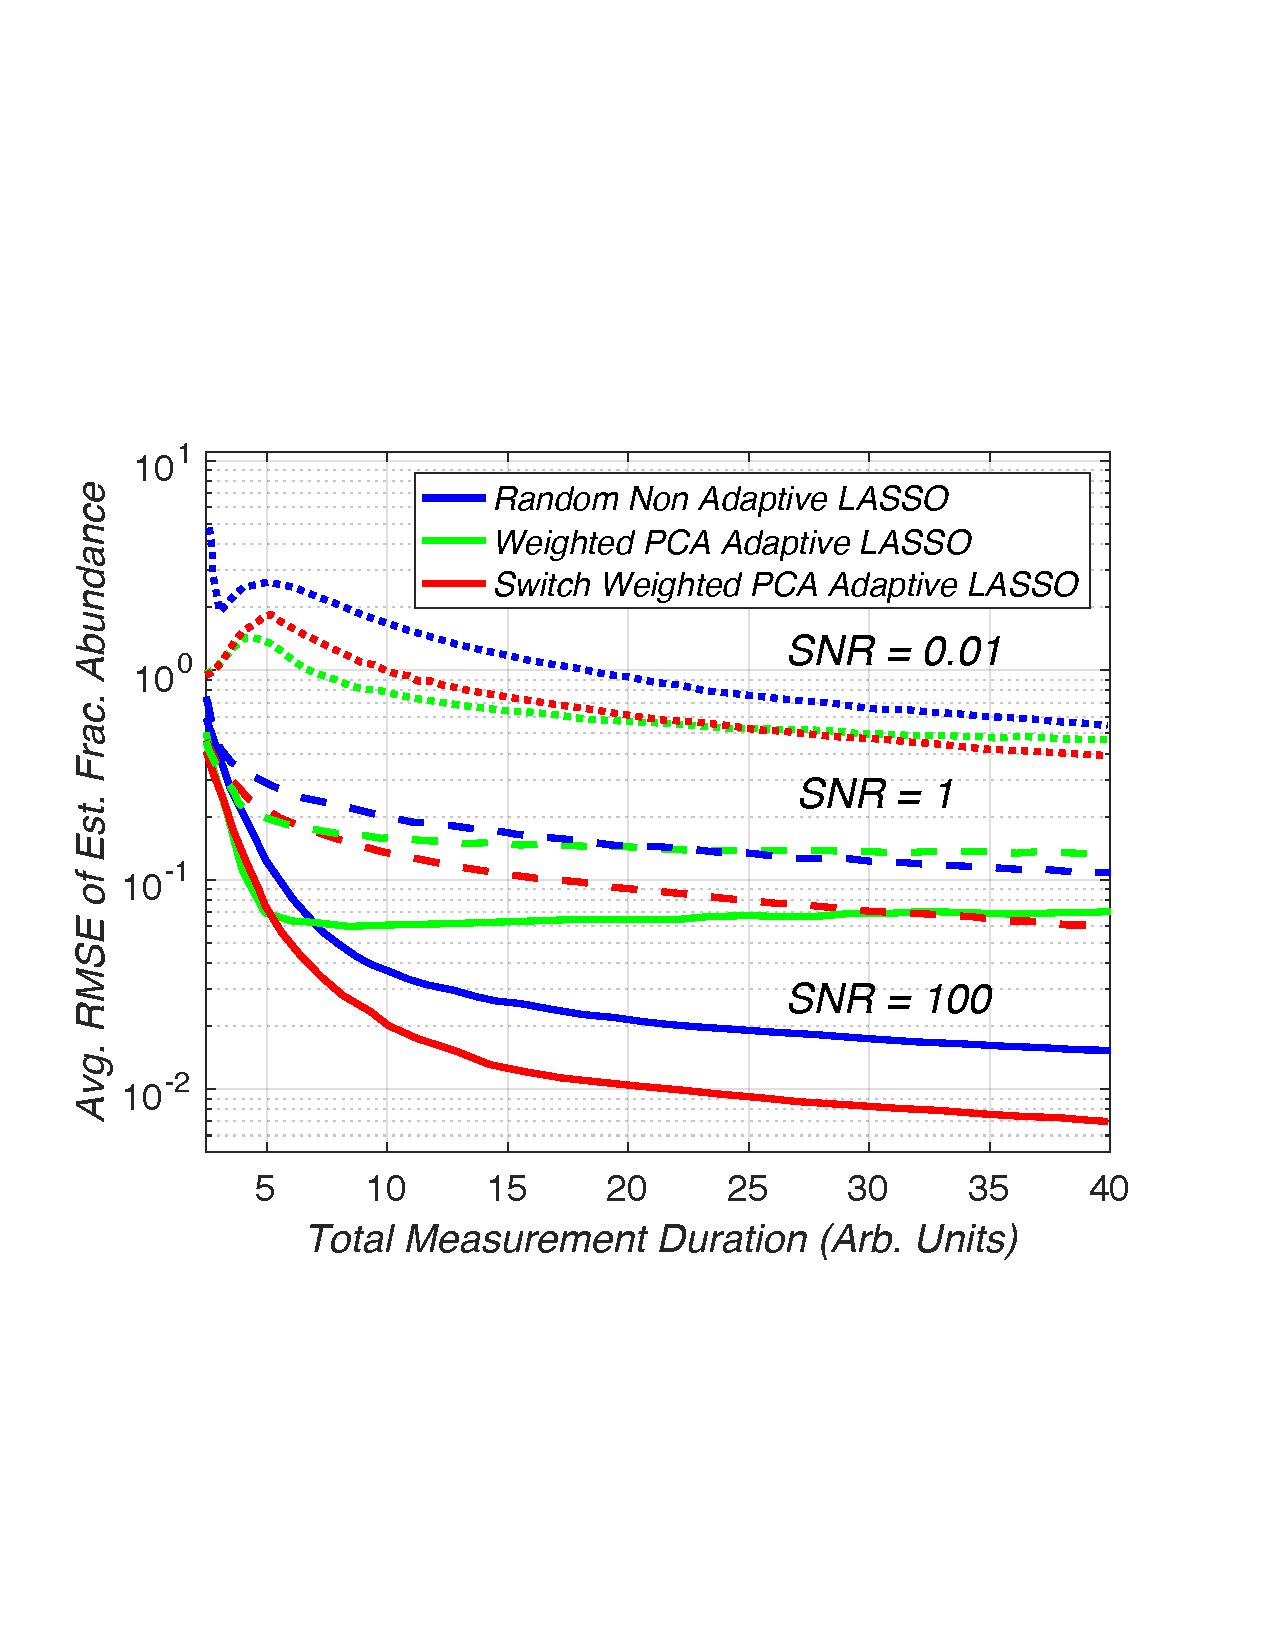
\includegraphics[scale=0.75]{unmixingVsMeasurement.pdf}
	\captionof{figure}[Comparison of Spectral Unmixing Techniques for the AFSSI-C versus Measurement Duration]{Comparison of Spectral Unmixing Techniques for the AFSSI-C versus Measurement Duration for SNR = 0.01, 1.0, and 100. Even though the spectral library is weighted by the fractional abundances from the last measurement, simply using every principal component underperforms using random spectral filters with $\ell_1$ regularized least squares (lasso). Switching the principal components according the algorithm described in \Cref{sec:unmixingAlgo} siginificantly reduces the unmixing error. }
	\label{fig:unmixingVsMeasurement}
\end{figure}


\subsection{Initial Experimental Results}

I developed an initial proof-of-principle experiment using the \gls{afssi-c} architecture. For this experiment I had to modify the \gls{afssi-c} prototype experiment by adding an second display. This is because the original prototype used only one LED computer monitor. So it can only display combinations of the same red, green, and blue (RGB) spectra. Therefore, it can only produce 3 endmembers in the library. Therefore, I added an OLED display which also has red, green, and blue spectra, but they different enough that are not simply scaled versions of the RGB spectra from the LED monitor. This is shown in \Cref{fig:unmixingLibrary}. Note that the RGB spectra from the LED look different from Figure BLAH BLAH BLAH because the transmission from the pelicle beam splitter. 

With the exception of the pellicle beam splitter, an achromatic doublet, and the OLED Display which is controlled through a USB connection to MATLAB, the experimental prototype is the same as the one used for spectral classificaiton. 

\begin{figure}
	\centering
	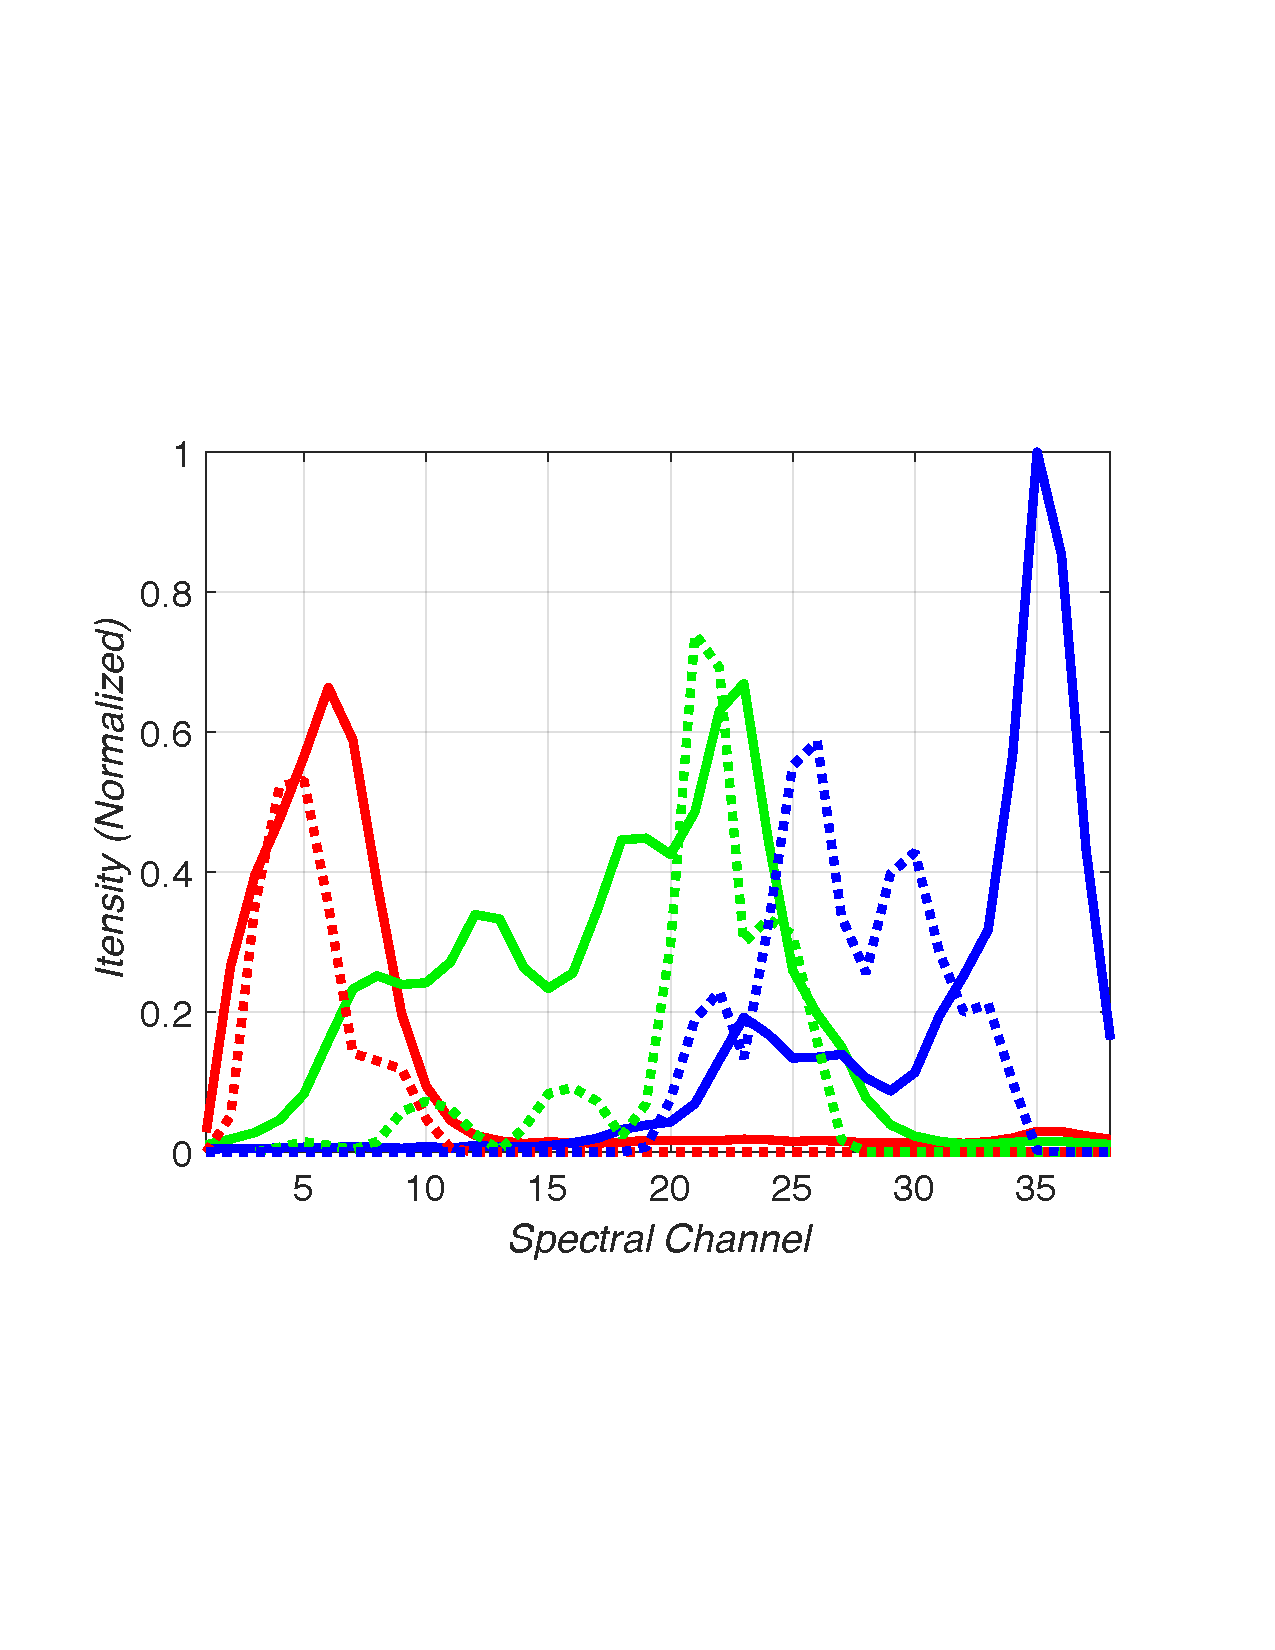
\includegraphics[scale=0.75]{unmixingLibrary}
	\captionof{figure}[Six Endmember Spectra Used For Spectral Unmixing Experiment]{The six endmember spectra used for the spectral unmixing experiment. The library consist of the red, green, and blue spectra from an LED Monitor and the red, green, and blue spectra from the OLED. The LED monitor spectra may look different from the one shown in Chapter 4 since the spectra have been modified by transmitting through a pellicle beam splitter. }
	\label{fig:unmixingLibrary}
\end{figure}

\begin{figure}
	\centering
	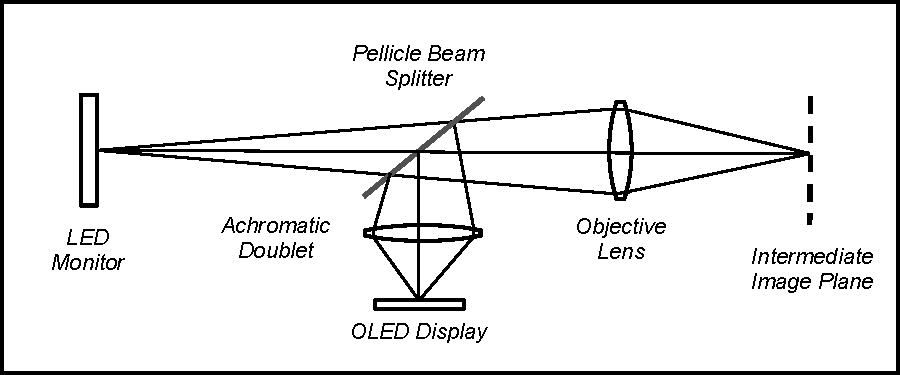
\includegraphics[scale=1.00]{unmixingArch1.pdf}
	\captionof{figure}[Unmixing Architecture for Spectral Unmixing Experiment]{Experimental architecture used to superimpose the spectral images from the LED monitor, which already was in place, and an OLED display. ZEMAX was used to find the correct location of the achromatic doublet, OLED display, and pellicle beam splitter to ensure the intermediate image from both displays appeared at the same location and with the same transverse magnification.}
	\label{fig:unmixingArch1}
\end{figure}

\begin{figure}
	\centering
	\includegraphics[scale=0.70]{solidworksOfMixingSetupPicture3.png}
	\captionof{figure}[Computer Aided Design (CAD) drawing of experimental mixing setup.]{Computer Aided Design (CAD) drawing of experimental mixing setup.}
	\label{fig:solidworksOfMixingSetupPicture3} 
\end{figure}


\begin{figure}
	\centering
	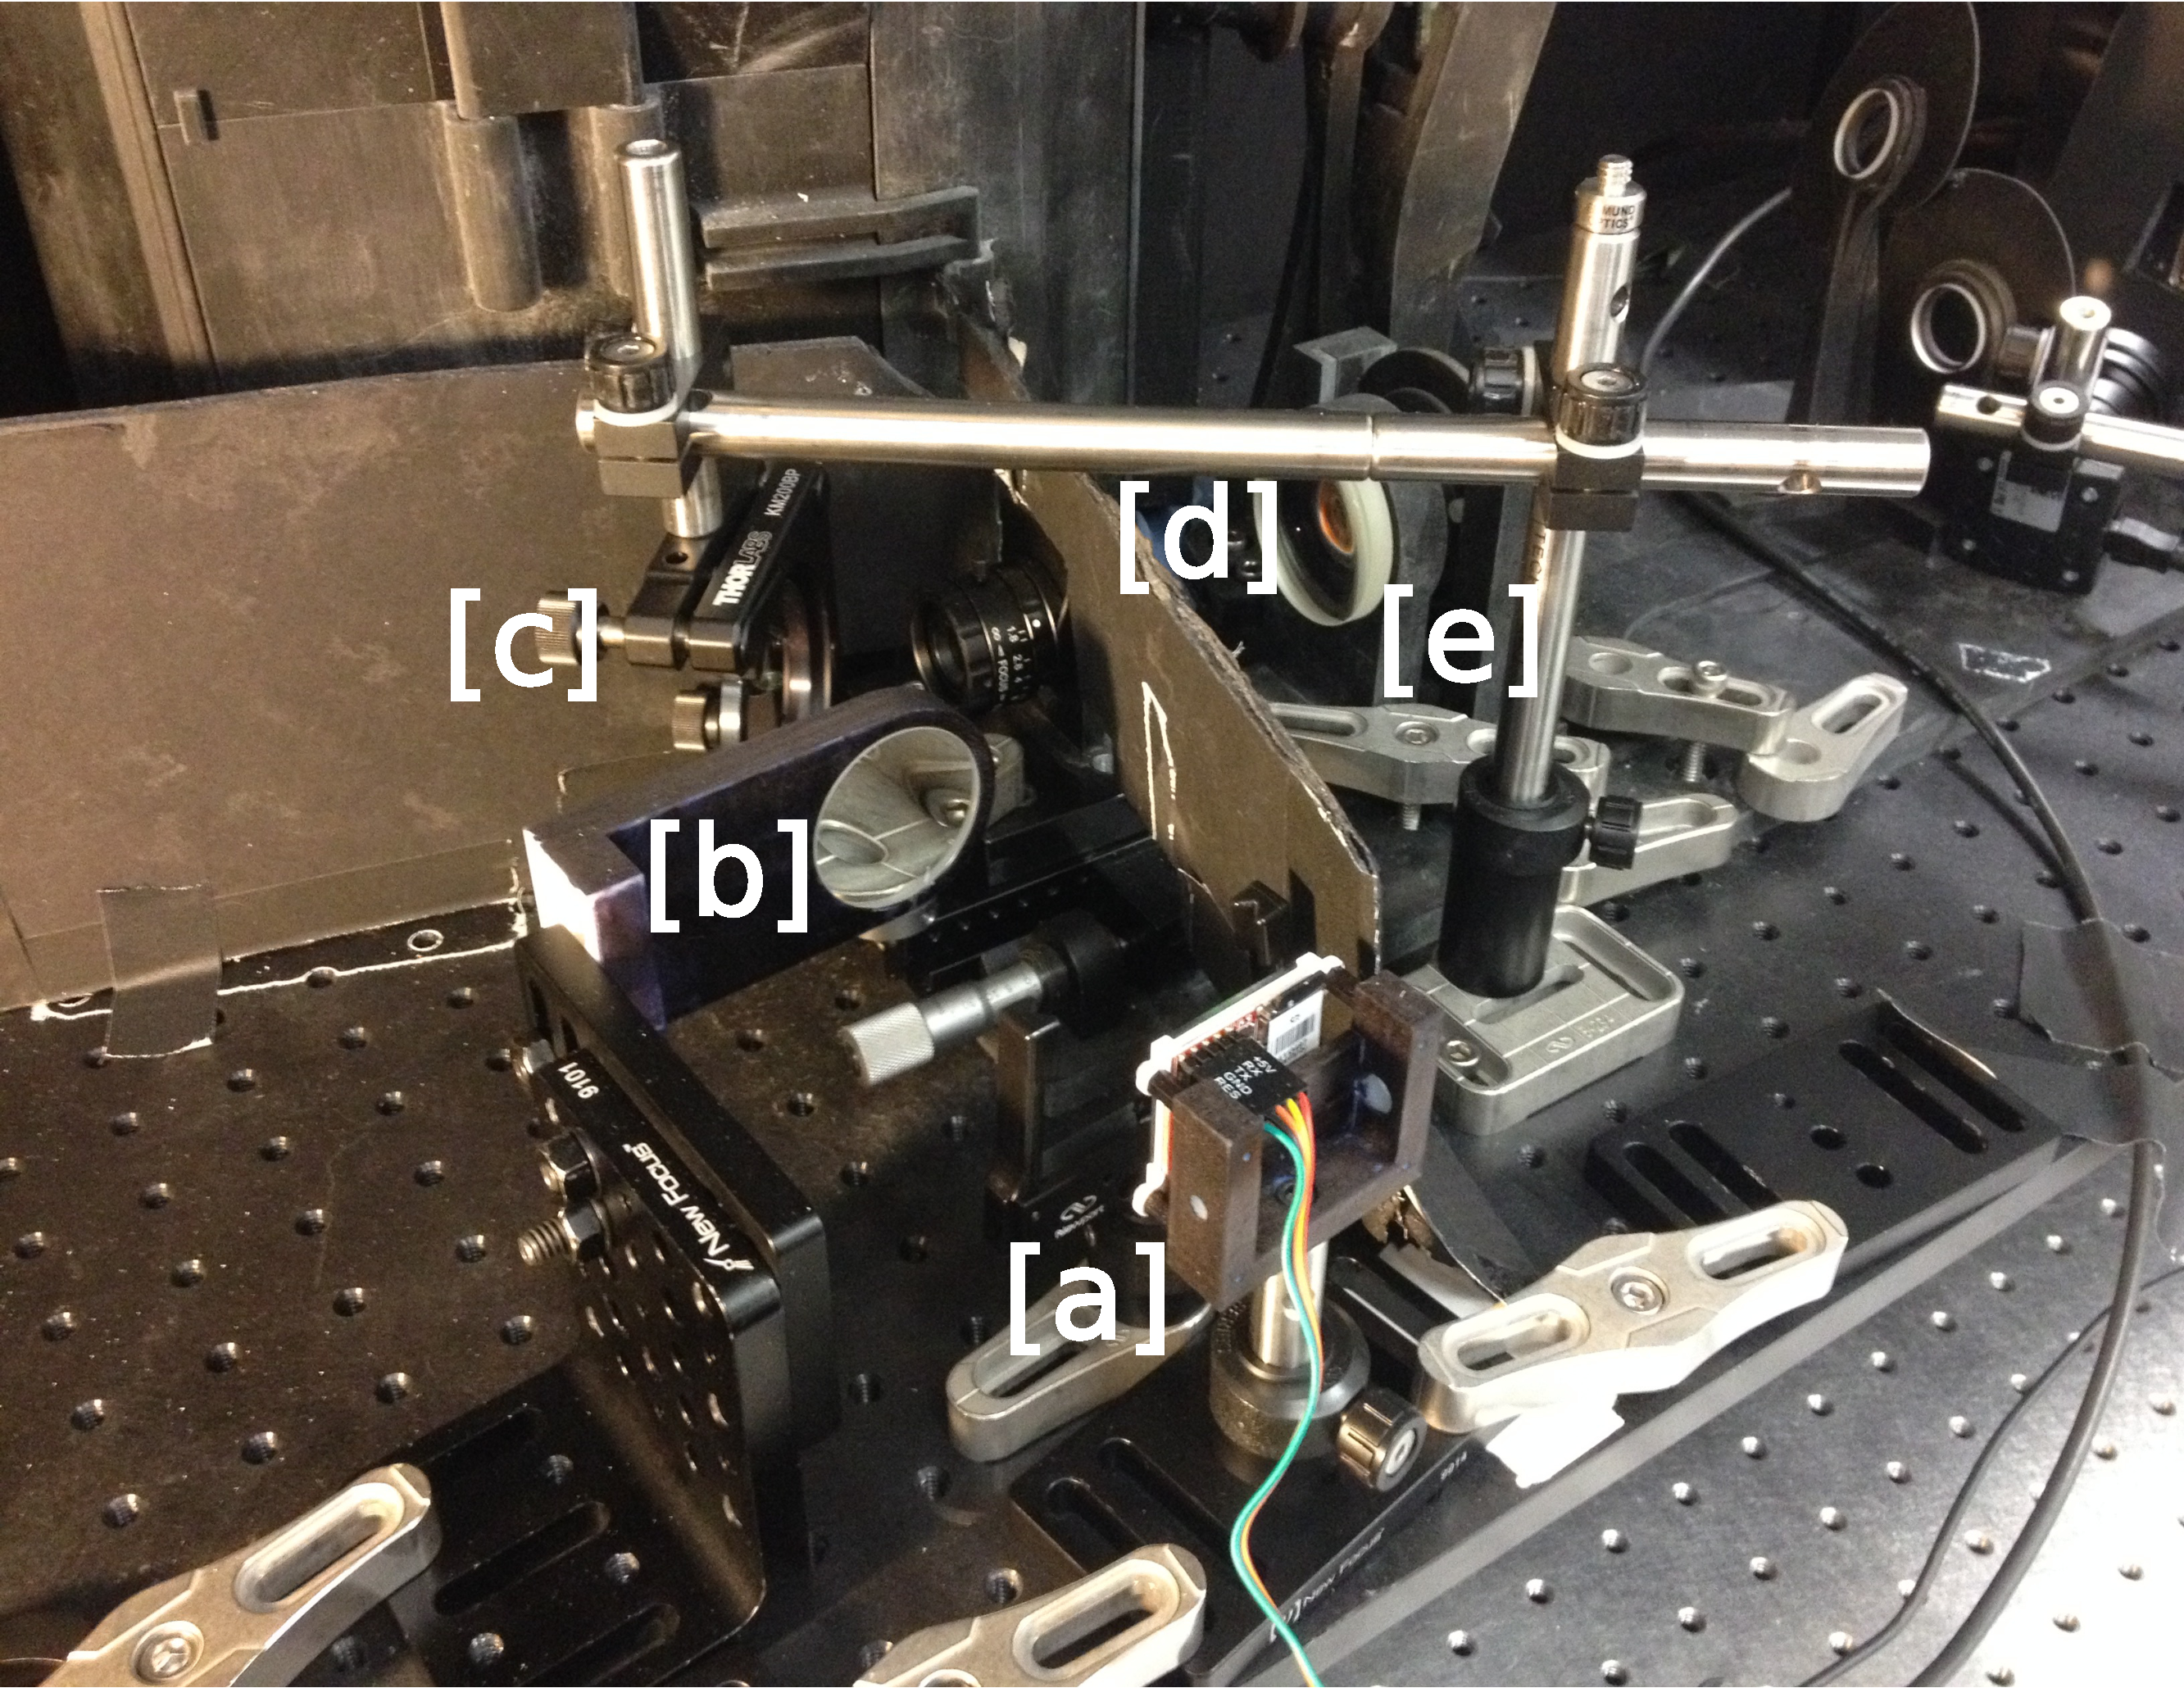
\includegraphics[scale=0.30]{unmixingSetupPhoto2.pdf}
	\captionof{figure}[Unmixing Architecture for Spectral Unmixing Experiment]{Photograph of the spectral unmixing experiment. (a) The OLED Display (b) Achromatic Doublet (c) Pellicle Beam Splitter (d) Objective Lens (e) First Lens of the AFSSI-C system. The intermediate image is located between the objective lens and the first lens of the system. Black foamboard is used to reduce stray light.}
	\label{fig:unmixingSetupPhoto2} 
\end{figure}

\begin{figure}
	\centering
	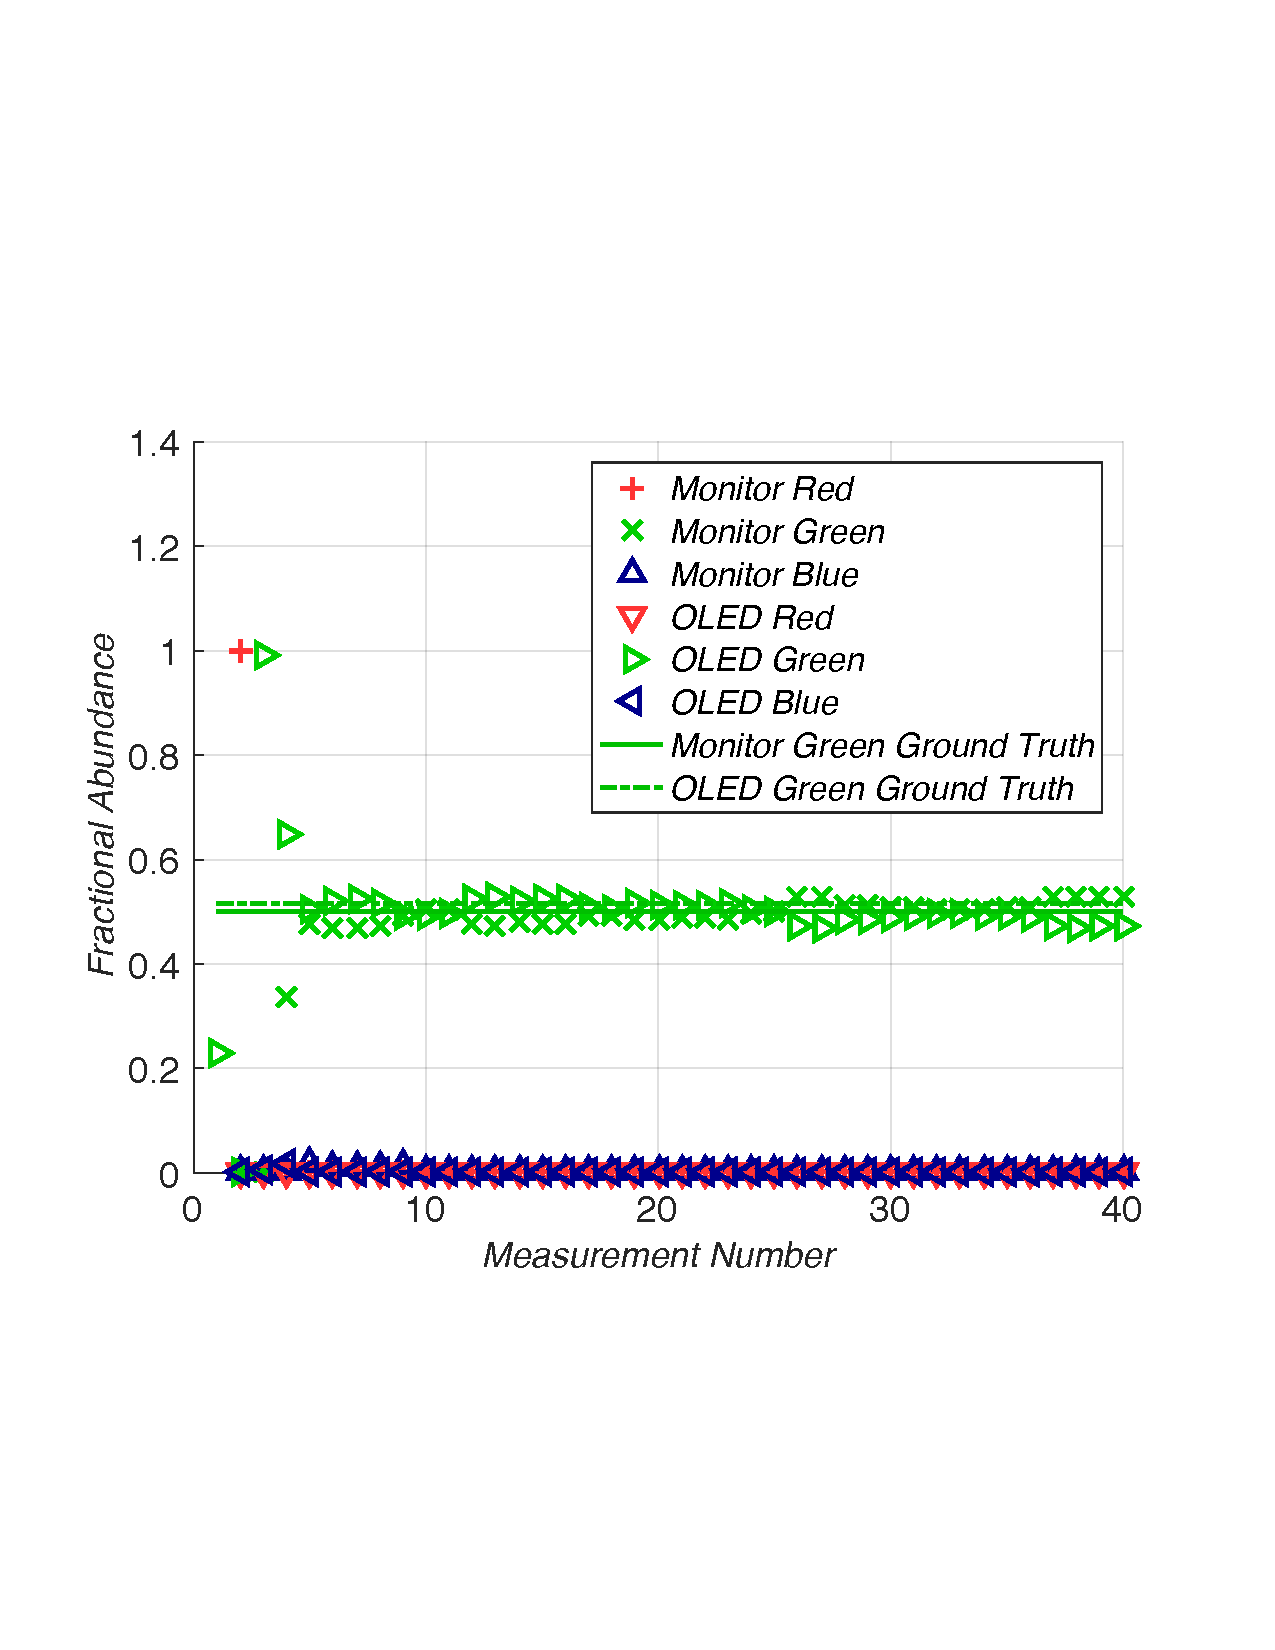
\includegraphics[scale=0.70]{unmixingResultLinearGreenRamp3232.pdf}
	\captionof{figure}[Single Pixel Experimental Spectral Unmixing Results Using the AFSSI-C]{Single Pixel Spectral Unmixing Results with the AFSSI-C with random binary spectral filters. The MATLAB \texttt{lasso} function correctly identifies fractional abundance of the two green spectra from each display within five measurement steps. The four other spectra are estimated to be zero. }
	\label{fig:unmixingResultLinearGreenRamp3232} 
\end{figure}

\begin{figure}
	\centering
	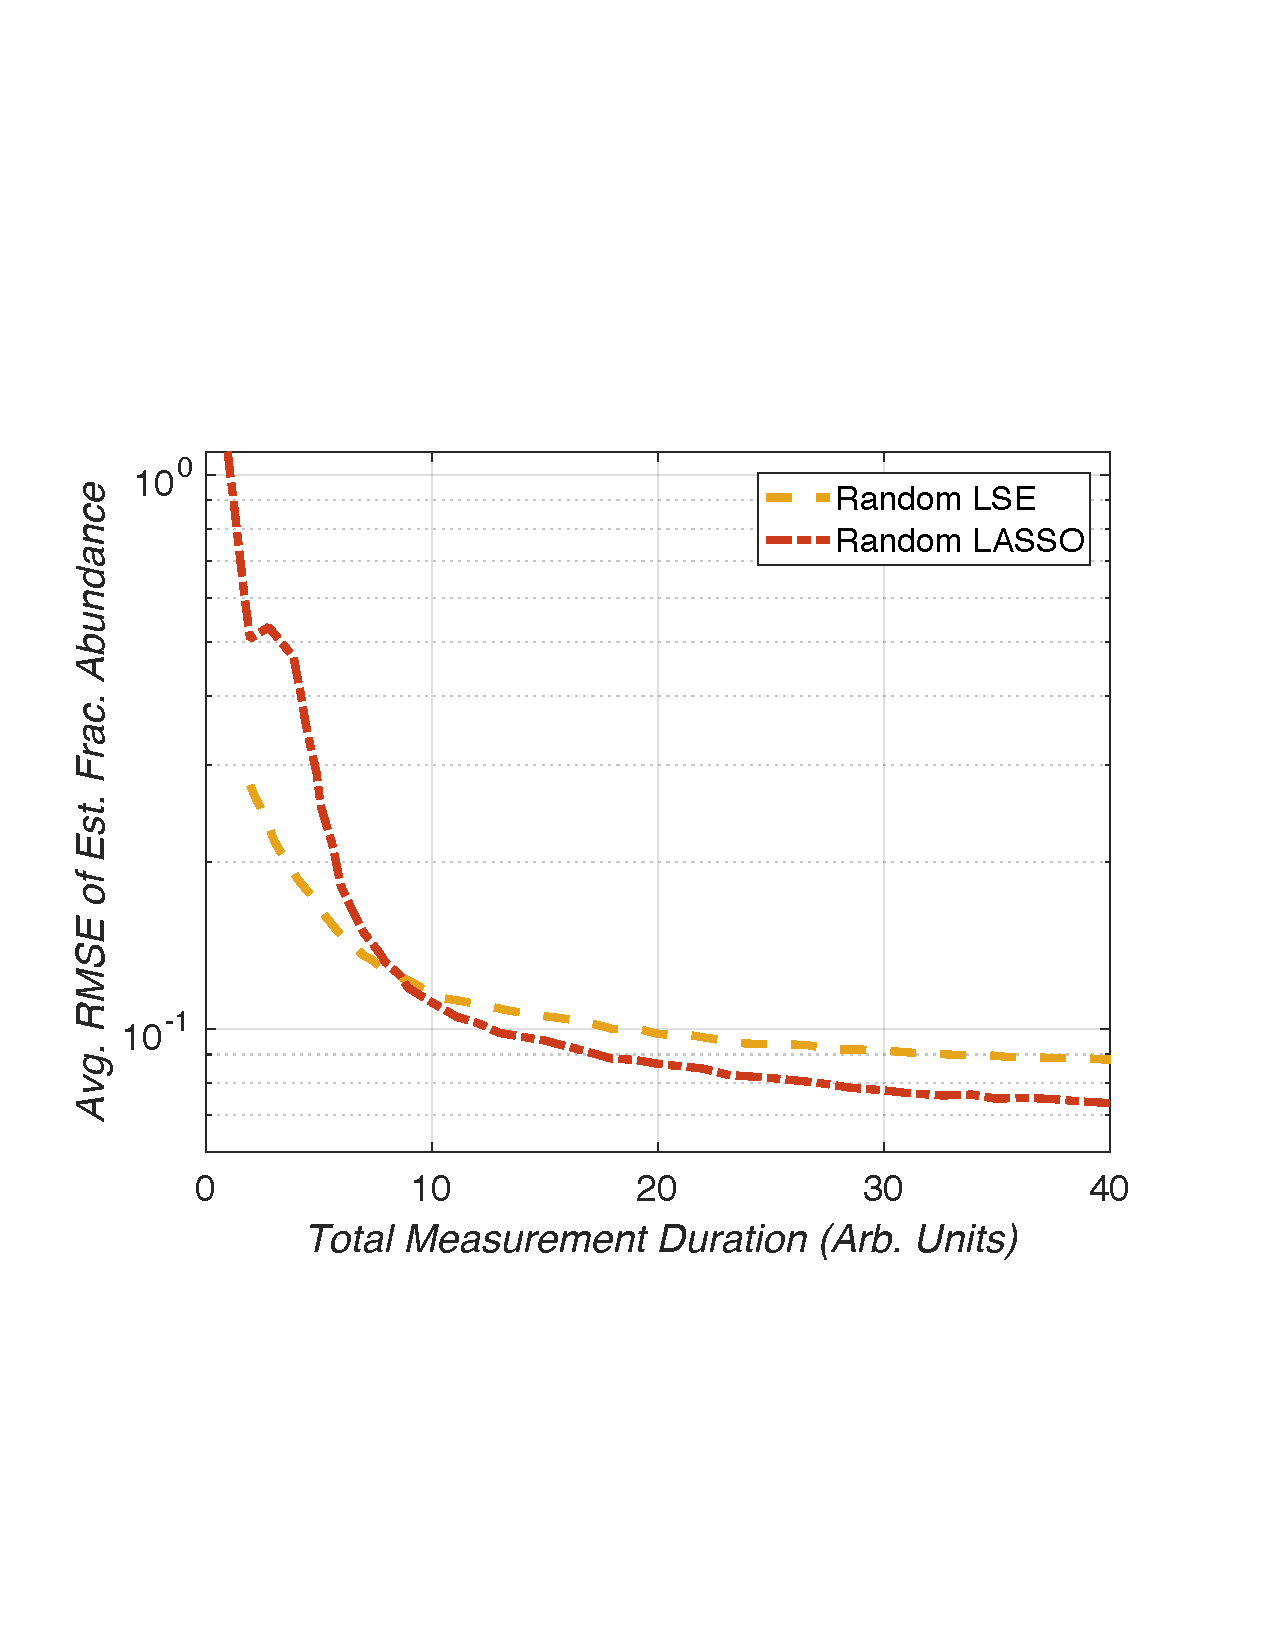
\includegraphics[scale=0.70]{rmseVsMeasurementExperiment.pdf}
	\captionof{figure}[32 $\times$ 32 Experimental Spectral Unmixing Results Using the AFSSI-C]{32 $\times$ 32 Experimental Spectral Unmixing Results Using the AFSSI-C with random binary spectral filters. The MATLAB \texttt{lasso} function outperforms the least squares estimator as the number of measurements increase. Thus have an opportunity to beat traditional systems using significantly fewer measurements}
	\label{fig:rmseVsMeasurementExperiment} 
\end{figure}


